% Use this template to write your solutions to COS 423 problem sets

\documentclass[12pt]{article}
\usepackage[utf8]{inputenc}
\usepackage{amsmath, amsfonts, amsthm, amssymb, algorithm, graphicx, mathtools, xfrac}
\usepackage[noend]{algpseudocode}
\usepackage{fancyhdr, lastpage}
\usepackage{booktabs}
\usepackage{multirow}
\usepackage{graphicx}
\usepackage{pgfplots}
\usepackage[vmargin=1.20in,hmargin=1.25in,centering,letterpaper]{geometry}
\setlength{\headsep}{.50in}
\setlength{\headheight}{15pt}

% Landau notation
\DeclareMathOperator{\BigOm}{\mathcal{O}}
\newcommand{\BigOh}[1]{\BigOm\left({#1}\right)}
\DeclareMathOperator{\BigTm}{\Theta}
\newcommand{\BigTheta}[1]{\BigTm\left({#1}\right)}
\DeclareMathOperator{\BigWm}{\Omega}
\newcommand{\BigOmega}[1]{\BigWm\left({#1}\right)}
\DeclareMathOperator{\LittleOm}{\mathrm{o}}
\newcommand{\LittleOh}[1]{\LittleOm\left({#1}\right)}
\DeclareMathOperator{\LittleWm}{\omega}
\newcommand{\LittleOmega}[1]{\LittleWm\left({#1}\right)}

% argmin and argmax
\newcommand{\argmin}{\operatornamewithlimits{argmin}}
\newcommand{\argmax}{\operatornamewithlimits{argmax}}

\newcommand{\calP}{\mathcal{P}}
\newcommand{\Z}{\mathbb{Z}}
\newcommand{\R}{\mathbb{R}}
\newcommand{\Exp}{\mathbb{E}}
\newcommand{\Q}{\mathbb{Q}}
\newcommand{\sign}{\mathrm{sign\ }}
\newcommand{\abs}{\mathrm{abs\ }}
\newcommand{\eps}{\varepsilon}
\newcommand{\zo}{\{0, 1\}}
\newcommand{\SAT}{\mathit{SAT}}
\renewcommand{\P}{\mathbf{P}}
\newcommand{\NP}{\mathbf{NP}}
\newcommand{\coNP}{\co{NP}}
\newcommand{\co}[1]{\mathbf{co#1}}
\renewcommand{\Pr}{\mathop{\mathrm{Pr}}}

% theorems, lemmas, invariants, etc.
\newtheorem{theorem}{Theorem}
\newtheorem{lemma}[theorem]{Lemma}
\newtheorem{invariant}[theorem]{Invariant}
\newtheorem{corollary}[theorem]{Corollary}
\newtheorem{definition}[theorem]{Definition}
\newtheorem{property}[theorem]{Property}
\newtheorem{proposition}[theorem]{Proposition}

% piecewise functions
\newenvironment{piecewise}{\left \{\begin{array}{l@{,\ }l}}
{\end{array}\right.}

% paired delimiters
\DeclarePairedDelimiter{\ceil}{\lceil}{\rceil}
\DeclarePairedDelimiter{\floor}{\lfloor}{\rfloor}
\DeclarePairedDelimiter{\len}{|}{|}
\DeclarePairedDelimiter{\set}{\{}{\}}

\makeatletter
\@addtoreset{equation}{section}
\makeatother
\renewcommand{\theequation}{\arabic{section}.\arabic{equation}}

% algorithms
\algnewcommand\algorithmicinput{\textbf{INPUT:}}
\algnewcommand\INPUT{\item[\algorithmicinput]}
\algnewcommand\algorithmicoutput{\textbf{OUTPUT:}}
\algnewcommand\OUTPUT{\item[\algorithmicoutput]}


% Formating Macros

\pagestyle{fancy}
\lhead{\sc \hmwkClass\ $\; \;\cdot \; \;$ \hmwkSemester\ $\; \;\cdot \; \;$
Problem \hmwkAssignmentNum.\hmwkProblemNum}
%\chead{\sc Problem \hmwkAssignmentNum.\hmwkProblemNum}
%\chead{}
\rhead{\em \hmwkAuthorName\ $($\hmwkAuthorID$)$\/}
\cfoot{}
\lfoot{}
\rfoot{\sc Page\ \thepage\ of\ \protect\pageref{LastPage}}
\renewcommand\headrulewidth{0.4pt}
\renewcommand\footrulewidth{0.4pt}

\fancypagestyle{fancycollab}
{
    \lfoot{\textit{Collaborators: \hmwkCollaborators}}
}

\fancypagestyle{problemstatement}
{
    \rhead{}
    \lfoot{}
}

%%%%%% Begin document with header and title %%%%%%%%%%%%%%%%%%%%%%%%%

\begin{document}

%%%%%% Header Information %%%%%%%%%%%%%%%%%%%%%%%%%%%%%%%%%%%%%%%%%%%

%%% Shouldn't need to change these
\newcommand{\hmwkClass}{COS 255}
\newcommand{\hmwkSemester}{Spring 2016}

%%% Your name, in standard First Last format
\newcommand{\hmwkAuthorName}{Lukas Leung}
%%% Your NetID
\newcommand{\hmwkAuthorID}{lleung}

%%% The problem set number (just the number)
\newcommand{\hmwkAssignmentNum}{6}

%%% The problem number (just the number)
\newcommand{\hmwkProblemNum}{2}

%%% A list of your collaborators' NetIDs, separated by ", ".
%%% You can use a new line ("\\") in the middle to prevent a long
%%% list from overflowing.
\newcommand{\hmwkCollaborators}{}
%%% Sets the collaborator list to appear on the first page
\thispagestyle{fancycollab}

%%%%%%% begin Solution %%%%%%%%%%%%%%%%%%%%%%%%%%%%%%%%%%%%%%%%%%%%
%\section{Results from UVA}
%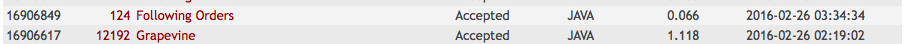
\includegraphics[width=\textwidth]{uvaResults}
%\newpage

%%%%%%% start Angry Programmer %%%%%%%%%%%%%%%%%%%%%%%%%%%%%%%%%%%%%%%%%%

\section{UVA Problem 11506: Angry Programmer}
\textbf{Background} \\
~\indent You, a programmer of an important software house, have been fired because you
didn't solve an important problem that was assigned to you. You are very furious
and want to take revenge on your boss, breaking the communication between his
computer
and the central server. \\
~\indent The computer of your boss and the central server are in the same network, which
is composed of many machines (computers) and wires linking pairs of those machines.
There is at most one wire between any pair of machines and there can be pairs of
machines without a wire between them. \\
~\indent To accomplish your objective, you can destroy machines and wires, but you can't
destroy neither the computer of your boss nor the central server, because those machines
are monitored by security cameras. You have estimated the cost of blowing up
each machine and the cost of cutting each wire in the network. \\
~\indent You want to determine the minimum cost of interrupting the communication between
your boss' computer and the central server. Two computers $A$ and $B$ can
communicate if there is a sequence of undestroyed machines $x_1,...,x_n$ such that
$x_1 = A, x_n = B$ and $x_i$ is linked with $x_{i+1}$ with an uncut wire (for each $1 \leq i \leq n - 1$). \\ \\
\textbf{Input} \\
The input consists of several test cases. Each test case is represented as follows:
\begin{itemize}
    \item A line with two integers $M$ and $W$ ($2 \leq M \leq 50, 0 \leq W \leq 1000$), representing
    (respectively) the number of machines and the number of wires in the network.
    \item \textbf{M-2} lines, one per machine (different from the boss' machine and the central
    server), containing the following information seperated by spaces:
    \begin{itemize}
        \item An integer $i\ (2 \leq i \leq M-1)$ with the identifier of the machine. Assume
        that the boss' machine has id 1 and that the central server has id $M$.
        \item An integer $c\ (0 \leq c \leq 100000)$ specifying the cost of destroying the machine.
    \end{itemize}
    \item \textbf{W} lines, one per wire, containing the following information separated by spaces:
    \begin{itemize}
        \item Two integers $j$ and $k\ (1 \leq j \textless k \leq M)$ specifying the identifiers of the machines linked by the wire. remember that the wire is bidirectional.
        \item An integer $d (0 \leq d \leq 100000)$ specifying the cost of cutting the wire.
    \end{itemize}
\end{itemize}
The end of the input is specified by a line with the string "0 0". \\
Suppose that the machines have distinct identifiers.

%%%%%%% end Problem %%%%%%%%%%%%%%%%%%%%%%%%%%%%%%%%%%%%%%%%%%%%%%%

\newpage

%%%%%%% Mathematical Formulation %%%%%%%%%%%%%%%%%%%%%%%%%%%%%%%%%%
\subsection{Mathematical Formulation}
Given an input of $M$ machines, $M-2$ of which are potential intermediate nodes
between the boss' computer and the server, and $W$ wires connecting computers $m_i$
and $m_j$ where $0 \leq i \textless j \leq M$, determine the minimum cost to destroy (m + w)
machines and wires where $(0 \leq m \leq M-2, 0 \leq w \leq W)$.

%%%%%%% Algorithm %%%%%%%%%%%%%%%%%%%%%%%%%%%%%%%%%%%%%%%%%%%%%%%%%

\subsection{Solution}
Important Confusing Data Structures:
\begin{itemize}
    \item LinkedList$\textless$FlowEdge$\textgreater$[ ] \textbf{adj} : ~ An adjacency list of all FlowEdges where the
    specified node is the originating node.
\end{itemize}

The main functionality of this algorithm is to implement the Ford Fulkerson min
cut algoritm by first building a flow network and then executingthe algorithm on it.
We represent the network as each machine (index) has its own linked list of Flow
Edges. Each computer has 2 nodes, one as its input and the other as its output. The
only edge that flows out of the input and into the output is the edge connecting the
two such that the input points to the output with edgeweight equivalent to the cost
of destroying that computer; this is the MAX\_INTEGER for the boss' computer and
the server since we cannot destroy these. Since we are given the boss' computer as
"1" and the server as "M" we just let the input for every computer be index = i-1
and their output as index = (i-1)+M for $i \in 1..M$ as described below.

\begin{algorithm}[H]
\caption{Determine index of Computers}
\begin{algorithmic}
    \Procedure{detIndex}{int index, boolean out}
        \If{out}
            return (index - 1) +  m
        \EndIf
        \State return (index - 1)
    \EndProcedure
\end{algorithmic}
\end{algorithm}

Once we do this we have to ensure that the bi-directional rule is accounted for.
So, for each wire connecting computers A and B with cost C, we will connect the
output for A to the input for B with weight C and the output of B to the input of A
with cost C. Once we have built up the entirety of our network we will simply use
the Ford Fulkerson algorithm on the built network and print that out. (As outlined
below)

\begin{algorithm}[H]
\caption{Build the Flow Network from input}
\begin{algorithmic}
    \Procedure{Main}{Scanner input}
        \While{true}
            \State $m, w \gets$ from input
            \If{m == 0 \&\& w == 0}
                break;
            \EndIf
            \If{w == 0}
                \State \Call{print}{0}
                \For{m-2 times}
                    input.\Call{nextLine}{ }
                \EndFor
            \EndIf
            \State $int numV,serverIn \gets$ 2*m, m-1 respectively
            \State $adj[numV] \gets$ initialized
            \State // create computers
            \State adj[0].\Call{add}{FlowEdge(0, m, Integer.MAX\_VALUE)}
            \State adj[serverIn].\Call{add}{FlowEdge(serverIn, numV-1, Integer.MAX\_VALUE)}
            \For{length of m-2}
                \State $int i, c \gets$ index of machine and cost to destroy
                \State $FlowEdge e \gets$ new FlowEdge(i, i+m, c)
                \State adj[i].\Call{add}{e}
            \EndFor
            \State // connect computers to eachother
            \For{length of W}
                \State $int a, b, c \gets$ comp1, comp2, cost to cut wire
                \State $outA, inA \gets$ detIndex(a, true), detIndex(a, false)
                \State $outB, inB \gets$ detIndex(b, true), detIndex(b, false)
                \State $e1, e2 \gets$ FlowEdge(outA, inB, c), FlowEdge(outB, inB)
            \EndFor
            \State \Call{print}{calcMinCut()}
        \EndWhile
    \EndProcedure
\end{algorithmic}
\end{algorithm}

%%%%%%% Correctness %%%%%%%%%%%%%%%%%%%%%%%%%%%%%%%%%%%%%%%%%%%%%%%

\subsection{Correctness}
%%%%%%% PROPOSITION 1 %%%%%%%%%%%%%%%
\begin{proposition}
~ \\ \indent This is the correct flow Network to build which will yeild the min cut.
\end{proposition}

\begin{proof}
~ \\ \indent This is correct because we are using the "flow" of each edge to be the cost of
destroying either a wire or a computer. We account for the fact that if we destroy
a computer, then we will also sever any connection that used this computer as an
intermediate node. We have done this by seperating each computer into an input and
an output node, between which $\exists$ only one connection which has a flow of the cost of
destroying a computer. The bi-directional aspects has us connect the network such
that, for each wire connecting computers A and B with cost C, we will connect the
output for A to the input for B with weight C and the output of B to the input of A
with cost C. Therefore if we sever inA to outA (destroying computer A) B would
no longer be able to use this as an intermedite node since inA no longer has any out
edges and outA is unreachable since its only in edge was just severed.
\end{proof}

%%%%%%% Analysis %%%%%%%%%%%%%%%%%%%%%%%%%%%%%%%%%%%%%%%%%%%%%%%%%%
\subsection{Analysis}
For the following analysis, we will say that we have built a flow network graph with
$V = 2\cdot M$ and $E = M + 2\cdot W$. Our Time and Space analysis will be done with these
variables but can be converted to V $\approx$ M and E $\approx$ (M+W)

%%%%%%% PROPOSITION 1 %%%%%%%%%%%%%%%
\begin{proposition}
\label{numq}
The \underline{space complexity} of this algorithm is \textbf{O(V+E)}
\end{proposition}

\begin{proof}
~ \\ \indent This is due to the fact that all of our data is stored in data structures:
\begin{itemize}
    \item \underline{adj[V]}: Our Flow NetWork $\implies V+E$
    \item \underline{edgeTo[V]}: Used in Ford Fulkerson implementation
\end{itemize}
\begin{center}
    Giving us a space complexity of \textbf{O(V+E)}
\end{center}
\end{proof}

%%%%%%% PROPOSITION 2 %%%%%%%%%%%%%%%
\begin{proposition}
\label{numq}
The \underline{time complexity} of this algorithm is \textbf{O(V+E+MaxFlowValue$\cdot$E)}
\end{proposition}

\begin{proof}
~ \\ \indent This is the case because our algorithm first builds our flow network which
takes V + E time and then implements the Ford Fulkerson Min Cut algorithm which
is synonomous to the Max Flow. This implementation takes MinCutValue$\cdot$E time.
\begin{center}
    Giving us a time complexity of \textbf{O(V+E+MaxFlowValue$\cdot$E)}
\end{center}
\end{proof}

%%%%%%% Example %%%%%%%%%%%%%%%%%%%%%%%%%%%%%%%%%%%%%%%%%%%%%%%%%%%

\subsection{An Example}
\textbf{input} \\
4 4   \\
3 5   \\
2 2   \\
1 2 3 \\
1 3 3 \\
2 4 1 \\
3 4 3 \\
0 0   \\
\\
Now when we run this through our Algorithm we will build first the nodes for the
computers and connect their "ins" to their "outs"
\begin{center}
(boss) $\implies$ 0 $\rightarrow$ 4 with cap = 2.147483647$\cdot10^9$   \\
(server) $\implies$ 3 $\rightarrow$ 7 with cap = 2.147483647$\cdot10^9$  \\
(3 5) $\implies$ 2 $\rightarrow$ 6 with cap = 5.0   \\
(2 2) $\implies$ 1 $\rightarrow$ 5 with cap = 2.0
\end{center}

\noindent Next we build the wire connections:

\begin{center}
(1 2 3) $\implies$ 4 $\rightarrow$ 1 with cap = 3.0 \\
convex $\implies$ 5 $\rightarrow$ 0 with cap = 3.0  \\ ~ \\
(1 3 3) $\implies$ 4 $\rightarrow$ 2 with cap = 3.0 \\
convex $\implies$ 6 $\rightarrow$ 0 with cap = 3.0  \\ ~ \\
(2 4 1) $\implies$ 5 $\rightarrow$ 3 with cap = 1.0 \\
convex $\implies$ 7 $\rightarrow$ 1 with cap = 1.0  \\ ~ \\
(3 4 3) $\implies$ 6 $\rightarrow$ 3 with cap = 3.0 \\
convex $\implies$ 7 $\rightarrow$ 2 with cap = 3.0
\end{center}

Then when we calculate the mincut value we get 4!




%%%%%%% end Angry Programmer %%%%%%%%%%%%%%%%%%%%%%%%%%%%%%%%%%%%%%%%%%%


%%%%%%% end Solution %%%%%%%%%%%%%%%%%%%%%%%%%%%%%%%%%%%%%%%%%%%%%%

\end{document}